\documentclass[../main.tex]{subfiles}
\graphicspath{{\subfix{../images/}}}
\usetikzlibrary{patterns}
\begin{document}
	\subsection{Rotacions}
	\subsubsection{L'espai euclidià estàndard 3-dimensional}
	Treballem a l'espai 3-dimensional en el qual vivim i que identifiquem amb $\mathbb{R}^3$.
	\begin{notacio}
	    En l'espai euclidià tenim l'origen a $\begin{psmallmatrix}0\\0\\0\end{psmallmatrix}$ i un punt
	    arbitrari $P = \begin{psmallmatrix}x\\y\\z\end{psmallmatrix} = \left(x,y,z\right) \in \mathbb{R}^3 = \mathbb{R} \times \mathbb{R} \times \mathbb{R}$.
	    Ambdues notacions (vertical i horitzontal) són vàlides malgrat representar diferents conceptes
	    tècnicament.
	\end{notacio}
	\begin{definicio}
	    La norma euclidiana d'un vector $V \in \mathbb{R}$ es defineix com
		\begin{displaymath}
			\left\lVert V\right\rVert = \sqrt{x^2+y^2+z^2} \in \mathbb{R}_+
		\end{displaymath}
	    que compleix $\forall V, W \in \mathbb{R}^3, \forall \lambda \in \mathbb{R}$
	    \begin{itemize}
	        \item $\left\lVert V+W\right\rVert \leq \left\lVert V\right\rVert + \left\lVert W\right\rVert$
	        \item $\left\lVert \lambda V\right\rVert = \left\lvert \lambda\right\rvert\left\lVert V\right\rVert$
	        \item $\left\lVert V\right\rVert = 0\iff V = 0$
	    \end{itemize}
	    Aquesta norma mesura la \underline{distància euclidiana} entre dos punts $P_1$ i $P_2$ per la fórmula
	    \begin{displaymath}
			\mathcal{D}\left(P_1, P_2\right) := \left\lVert P_1 - P_2\right\rVert = \sqrt{\left(x_1-x_2\right)^2 + \left(y_1-y_2\right)^2 + \left(z_1-z_2\right)^2}
		\end{displaymath}
		que compleix les seguents propietats
	    \begin{itemize}
	        \item $\mathcal{D}\left(P_1, P_3\right) \leq \mathcal{D}\left(P_1, P_2\right) + \mathcal{D}\left(P_2, P_3\right)$
	        \item $\mathcal{D}\left(P_1, P_2\right) = \mathcal{D}\left(P_2, P_1\right)$
	        \item $\mathcal{D}\left(P_1, P_2\right) = 0 \iff P_2 = P_1$
	    \end{itemize}
	\end{definicio}
	\begin{obs}
	    La norma euclidiana d'un vector $V$ correspon exactament a la seva longitud.
	\end{obs}
	\begin{demostracio}
	    Recordem el teorema de Pitàgores.\\
		\begin{center}
			\tikz[baseline={([yshift={-2.4*\ht\strutbox}]current bounding box.north)}] {
			\draw (0,0) -- (2,0) -- (2,1.5) -- cycle;
			\node at (1, -0.2) {$a$};
			\node at (2.2, 0.75) {$b$};
			\node at (0.8, 0.85) {$c$};
			\node at (1.25, 0.45) {$T$};
			\draw (2,0) rectangle (1.8,0.2);
			}
			\hspace{2em}$a^2+b^2=c^2$
		\end{center}
		Com
		\begin{center}
			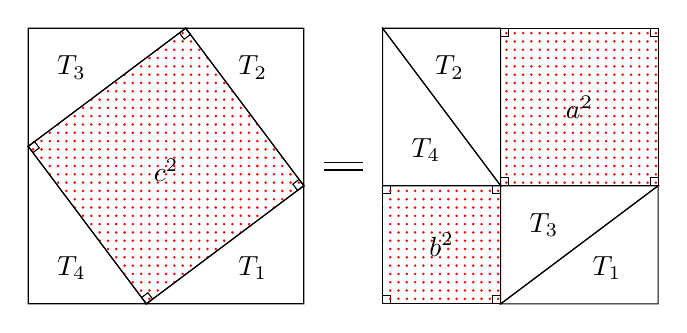
\begin{tikzpicture}
				%Primer cuadrat
				%Triangles
				\draw (0,0) -- (3.5,0) -- (3.5,3.5) -- (0,3.5) -- cycle;
				\draw (1.5,0) -- (3.5,0) -- (3.5,1.5) -- cycle;
				\node at (2.85, 0.45) {$T_1$};
				\draw (2,3.5) -- (3.5,3.5) -- (3.5,1.5) -- cycle;
				\node at (2.85, 3) {$T_2$};
				\draw (0, 2) -- (0, 3.5) -- (2, 3.5) -- cycle;
				\node at (0.55, 3) {$T_3$};
				\draw (0,0) -- (1.5,0) -- (0,2) -- cycle;
				\node at (0.55, 0.45) {$T_4$};
				%Angles de 90 graus
				\draw (1.5,0) -- (1.58,0.06) -- (1.52,0.14) -- (1.44,0.08) -- cycle;
				\draw (0,2) -- (0.08,2.06) -- (0.14,1.98) -- (0.06,1.92) -- cycle;
				\draw (2,3.5) -- (2.06,3.42) -- (1.98, 3.36) -- (1.92, 3.44) -- cycle;
				\draw (3.5,1.5) -- (3.44,1.58) -- (3.36,1.52) -- (3.42,1.44) -- cycle;
				%Area cuadrat
				\draw[pattern=dots, pattern color=red] (1.5,0) -- (0, 2) -- (2, 3.5) -- (3.5, 1.5) -- cycle;
				\node at (1.75, 1.7) {$c^2$};
				%Igualtat
				\draw (3.75, 1.8) -- (4.25, 1.8);
				\draw (3.75, 1.7) -- (4.25, 1.7);
				%segon cuadrat
				%Triangles
				\draw (6,0) -- (8,0) -- (8,1.5) -- cycle;
				\node at (7.35, 0.45) {$T_1$};
				\draw (4.5,3.5) -- (6,3.5) -- (6,1.5) -- cycle;
				\node at (5.35, 3) {$T_2$};
				\draw (6, 0) -- (6, 1.5) -- (8, 1.5) -- cycle;
				\node at (6.55, 1) {$T_3$};
				\draw (4.5,1.5) -- (6,1.5) -- (4.5,3.5) -- cycle;
				\node at (5.05, 1.95) {$T_4$};
				%Angles de 90 graus
				\draw (4.5,1.5) rectangle (4.6,1.4);
				\draw (4.5,0) rectangle (4.6,0.1);
				\draw (6,1.5) rectangle (5.9,1.4);
				\draw (6,0) rectangle (5.9,0.1);
				\draw (6,1.5) rectangle (6.1,1.6);
				\draw (8,1.5) rectangle (7.9,1.6);
				\draw (8,3.5) rectangle (7.9,3.4);
				\draw (6,3.5) rectangle (6.1,3.4);
				%Area cuadrat
				\draw[pattern=dots, pattern color=red] (4.5,0) rectangle (6,1.5);
				\draw[pattern=dots, pattern color=red] (6,1.5) rectangle (8,3.5);
				\node at (5.25, 0.75) {$b^2$};
				\node at (7, 2.5) {$a^2$};
			\end{tikzpicture}
		\end{center}
		Aleshores, veiem que $\left\lVert V\right\rVert$ és exactament
	    aplicar el teorema de Pitàgores dos cops, tal que
		\begin{center}
			\tikz[baseline={([yshift={-5*\ht\strutbox}]current bounding box.north)}] {
				\draw[->, thick, color = violet] (0,0) -- (3,3);
				\draw (0,0) -- (2,0) -- (2,2.5) -- (0,2.5) -- cycle;
				\draw (2,0) -- (3,0.5) -- (3,3) -- (2,2.5) -- cycle;
				\draw (0,2.5) -- (1,3);
				\draw (1,3) -- (3,3);
				\node at (1, -0.25) {$V_1$};
				\node at (-0.25, 1.25) {$V_2$};
				\node at (2.8, 0.1) {$V_3$};
				\node[color = violet] at (1, 1.25) {$V$};
			}
			$\;V =
				\begin{pmatrix}
					V_1\\
					V_2\\
					V_3
				\end{pmatrix}
			$
		\end{center}
		\begin{center}
			\tikz[baseline={([yshift={-5*\ht\strutbox}]current bounding box.north)}] {
				\draw[thick, color = violet] (0,0) -- (3,3);
				\draw[thick, color = red] (0,0) -- (3,0.5);
				\draw (3,0.5) rectangle (2.9,0.6);
				\draw (0,0) -- (2,0) -- (2,2.5) -- (0,2.5) -- cycle;
				\draw (2,0) -- (3,0.5) -- (3,3) -- (2,2.5) -- cycle;
				\draw (0,2.5) -- (1,3);
				\draw (1,3) -- (3,3);
				\node at (1, -0.25) {$V_1$};
				\node at (3.25, 1.5) {$V_2$};
				\node at (2.8, 0.1) {$V_3$};
				\node[color = violet] at (1, 1.35) {$L$};
				\node[color = red] at (1.75, 0.5) {$d$};
			}
			$\begin{cases}
			d^2 = V_1^2+V_2^2\\
			L^2 = d^2 + V_3^2
			\end{cases}
			\Rightarrow
			L^2 = V_1^2+V_2^2+V_3^2 = \left\lVert V\right\rVert^2$
		\end{center}
		Com la norma d'un vector $V \in \mathbb{R}^3$ correspon a la seva longitud, de forma equivalent la
		distància entre dos punts a $\mathbb{R}^3$ correspon a la longitud del segment que uneix aquests punts:\\
		\begin{center}
			\begin{tikzpicture}
				\draw[color = violet] (0,0) -- (3,0);
				\draw[color = violet,->] (1.4,-0.5) -- (3,-0.5);
				\draw[color = violet,->] (1.6,-0.5) -- (0,-0.5);
				\draw[fill] (0,0) circle (0.025);
				\draw[fill] (3,0) circle (0.025);
				\node at (0,0.25) {$P_1$};
				\node at (3,0.25) {$P_2$};
				\node[color = violet] at (1.5,-0.75) {$\left\lVert P_2-P_1\right\rVert$};
			\end{tikzpicture}
		\end{center}
		Si tenim $P_1\text{ i }P_2$ punts que defineixen un segment, la longitud $\mathcal{D}\left(P_1, P_2\right) = \left\lVert P_2-P_1\right\rVert$\\
		Per tant, la distància euclidiana entre dos punts és la que coneixem!
	\end{demostracio}
	Aquesta norma (i distància) euclidiana prové d'una estructura que a més de les longituds conté la
	noció d'ortogonalitat:
	\begin{definicio}
	    Anomenem producte escalar a $\mathbb{R}^3$ la funció\\
	    $\left\langle\dots, \dots\right\rangle: \mathbb{R}^3 \times \mathbb{R}^3 \to \mathbb{R}$\\
	    $\left(V, W\right) \mapsto \left\langle V, W\right\rangle = V_1W_1 + V_2W_2 + V_3W_3$
	    que és
	    \begin{itemize}
	        \item Bilineal: $\left\langle V+\lambda \bar{V}, W\right\rangle = \left\langle V, W\right\rangle + \lambda\left\langle \bar{V}, W\right\rangle$ ídem si $V \leftrightsquigarrow W$
	        \item Simètrica: $\left\langle V, W\right\rangle = \left\langle W, V\right\rangle$
	        \item Definit positiu: $\left\langle V, V\right\rangle > 0$ si $V \neq 0$
	    \end{itemize}
	\end{definicio}
	Observem que $\forall V \in \mathbb{R}^3,\;\left\lVert V\right\rVert = \sqrt{\left\langle V, V\right\rangle}$:
	la norma es pot definir en funció del producte escalar.\\
	Recíprocament, veiem fàcilment la \underline{Identitat de Polarització}
	\begin{displaymath}
	    \left\langle V, W\right\rangle = \frac{1}{2}\left(\left\lVert V+W\right\rVert^2 - \left\lVert V\right\rVert^2 - \left\lVert W\right\rVert^2\right)\\
	    \forall V, W \in \mathbb{R}^3
	\end{displaymath}
	\begin{exercici}
	    Arribar a la Identitat de Polarització a partir d'allò.
	\end{exercici}
	El producte escalar permet definir la noció d'ortogonalitat. Per veure això, necessitem primer el
	resultat següent:
	\begin{teorema}[Desigualtat de Cauchy-Schwartz]
	    \begin{displaymath}
	        \forall V, W \in \mathbb{R}^3, \left\lvert \left\langle V, W\right\rangle \right\rvert \leq \left\lVert V\right\rVert \left\lVert W\right\rVert
	    \end{displaymath}
	    A més, la igualtat s'assoleix només si $\exists \lambda \in \mathbb{R}: V = \lambda W$
	\end{teorema}
	\begin{demostracio}
	    Fixem $V, W \in \mathbb{R}^3$ qualsevol. Aleshores definim $\forall\lambda\in\mathbb{R}$\\$\mathcal{P}(\lambda):=\left\lVert V+\lambda W\right\rVert^2 \geq 0$\\
	    Observem que $\mathcal{P}(\lambda)=\left\langle V+\lambda W, V+\lambda W\right\rangle = \left\lVert V\right\rVert^2 + 2\lambda\left\langle V,W\right\rangle + \lambda^2\left\lVert W\right\rVert^2 \Rightarrow \mathcal{P}$
	    és un polinomi en $\lambda$ de grau $2$. Llavors $\Delta = 4\left(\left\langle V,W\right\rangle^2 - \left\lVert V\right\rVert^2\left\lVert W\right\rVert^2\right)$ ha de ser $\leq 0$, ja que $\mathcal{P} \geq 0$.\\
	    Deduïm que $\Delta \leq 0 \iff \left\langle V, W\right\rangle^2-\left\lVert V\right\rVert^2\left\lVert W\right\rVert^2 \leq 0 \iff \left\langle V, W\right\rangle^2\leq\left\lVert V\right\rVert^2\left\lVert W\right\rVert^2$\\
	    Si $\Delta = 0$ això implica que $\exists \lambda_0 \in \mathbb{R} : \mathcal{P}\left(\lambda_0\right) = 0$, aleshores $\mathcal{P}\left(\lambda_0\right) = 0 \iff \left\lVert V+\lambda_0 W\right\rVert = 0 \iff V = - \lambda_0 W$
	\end{demostracio}
	Com a conseqüència, obtenim que el número
	\begin{displaymath}
	    \frac{\left\langle V, W\right\rangle}{\left\lVert V\right\rVert\left\lVert W\right\rVert } \in \left[-1, 1\right]\;\;\forall V, W \in \mathbb{R}^3\setminus\left\{0\right\}
	\end{displaymath}
	\begin{displaymath}
	    \left(\iff \left\lvert \left\langle V, W\right\rangle \right\rvert\leq\left\lVert V\right\rVert\left\lVert W\right\rVert\right)
	\end{displaymath}
	\begin{definicio}
	    L'únic $\theta \in \left[0, \pi\right] : \cos{\theta} = \frac{\left\langle V, W\right\rangle}{\left\lVert V\right\rVert\left\lVert W\right\rVert }$
	    s'anomena angle euclidià entre $V\text{ i }W$.
	\end{definicio}
	L'angle és efectivament l'angle que coneixem.\\
	Si $V = (1,0,0)\text{ i }W = (\cos{\alpha}, \sin{\alpha}, 0)$ obtenim que $\cos{\theta} = \frac{\left\langle V, W\right\rangle}{\left\lVert V\right\rVert\left\lVert W\right\rVert } = \frac{\cos{\alpha}}{1\times1} = \cos{\alpha} \Rightarrow \theta = \alpha$
	\begin{definicio}
	    Diem que $V\text{ i }W$ són ortogonals si $\left\langle V, W\right\rangle = 0$ o, de forma
	    equivalent, si l'angle entre $V\text{ i }W$ és $\frac{\pi}{2}$.\\
	    \begin{notacio}
	        Denotem dos vectors ortogonals entre si com $V\perp W$
	    \end{notacio}
	    Un conjunt de 3 vectors és base ortogonal si $\left\langle U, V\right\rangle = \left\langle V, W\right\rangle = \left\langle U, W\right\rangle = 0$,
	    És base ortonormal, si és base ortogonal i a més $\left\lVert U\right\rVert = \left\lVert V\right\rVert = \left\lVert W\right\rVert = 1$.
	\end{definicio}
	$\mathbb{R}^3$ admet una estructura addicional que permet multiplicar dos vectors:
	\begin{definicio}
	    $\forall V, W \in \mathbb{R}^3$, definim el seu producte vectorial
	    \begin{displaymath}
	        V\wedge W = \begin{psmallmatrix}
	        V_2W_3-V_3W_2\\
	        V_3W_1-V_1W_3\\
	        V_1W_2-V_2W_1
	        \end{psmallmatrix} \in \mathbb{R}^3
	    \end{displaymath}
	    que compleix
	    \begin{itemize}
	        \item Bilinealitat: $(U + \lambda V) \wedge W = U\wedge W + \lambda V\wedge W$ ídem a la
	        dreta.
	        \item Antisimètria: $V\wedge W = -W \wedge V$
	    \end{itemize}
	\end{definicio}
	Veiem fàcilment que $\forall V, W \in \mathbb{R}^3$ $\left\langle V\wedge W, V\right\rangle = 0 = \left\langle V\wedge W, W\right\rangle$
	Més enllà
	\begin{proposition}
	    $\forall U, V, W \in \mathbb{R}^3, \left\langle U, V\wedge W\right\rangle = \det{\left(U, V, W\right)}$
	\end{proposition}

	\subsubsection{Moviments rígids i grup ortogonal}

	Observar un objecte que es desplaça és equivalent que desplaçar-se observant aquest objecte fix. La visió 3D utilitza l'observació d'un mateix objecte des de 2 punts de vista $\neq$ (un per cada ull). Però això equival estrictament a l'observació d'un mateix objecte desplaçant-se a l'espai.\\
	Per això primer estudiarem aquestes transformacions de l'espai que preserven un objecte (s'anomenen moviments rígids). Són transformacions que preserven les distàncies entre qualsevol parell de punts de l'objecte.\\
	Comencem estudiant un conjunt particular de transformació a l'espai.

	\begin{definicio}
	    El grup ortogonal és el conjunt d'aplicacions lineals que preserven el producte escalar:
	    \begin{displaymath}
	        O(3) := \left\{M \in \mathcal{M}_3\left(\mathbb{R}\right) | \left\langle MV, MW \right\rangle = \left\langle V, W\right\rangle \forall V, W \in \mathbb{R}^3 \right\}
	    \end{displaymath}
	\end{definicio}

	\begin{obs}
	    Si $M \in O(3)$ i $V \in \mathbb{R}^3$, $\left\lVert MV\right\rVert = \left\lVert V\right\rVert$\\
	    Si $M\in O(3)$ i $V\perp W \Rightarrow MV \perp MW$
	\end{obs}

	Com $\forall V, W \in \mathbb{R}^3$, $\left\langle MV, MW\right\rangle = V^tM^tMW$ per tant,
	\begin{displaymath}
	    M \in O(3) \Leftrightarrow M^tM = \mathbb{I}_3
	\end{displaymath}
	Al final obtenim
	\begin{displaymath}
	    O(3) = \left\{M \in \mathcal{M}_3\left(\mathbb{R}\right) | M^tM = \mathbb{I}_3\right\}
	\end{displaymath}

	\begin{proposicio}
	    Si $M \in O(3)$, llavors $\det\left(M\right) = \pm 1$
	\end{proposicio}

	\begin{definicio}
	    Es defineix el grup especial ortogonal
	    \begin{displaymath}
	        SO(3) := \left\{M \in O(3) | \det{M} = 1\right\}
	    \end{displaymath}
	\end{definicio}

	Per construcció els elements de $SO(3)$ són aquestes transformacions lineals que preserven les
	bases ortogonals positives. És a dir, són aquestes que preserven l'orientació i més concretament,
	$\left(Me_1, Me_2, Me_3\right)$ compleix

	\begin{enumerate}
	    \item $\left(Me_1, Me_2, Me_3\right)$ és una base ortogonal
	    \item $\det{\left(Me_1, Me_2, Me_3\right)} = \det{M} = 1$ i doncs $\left\langle Me_1\wedge Me_2, Me_3\right\rangle = 1 \Rightarrow Me_3 = Me_1\wedge Me_2$
	\end{enumerate}

	Un exemple de $M \in O(3)\setminus SO(3)$ és la matriu $M = \begin{psmallmatrix}
	    1 & 0 & 0\\
	    0 & 1 & 0\\
	    0 & 0 & 1
	\end{psmallmatrix}$\\

	Aquestes transformacions de $O(3)\setminus SO(3)$ canvien l'orientació no corresponen al context de
	la visió 3D com no podem canviar l'orientació d'un objecte desplaçant-ho a l'espai. Per això tindrem
	especial èmfasi en el subgrup $SO(3)$!

	\begin{obs}
	    $O(3)$ i $SO(3)$ són grups (noció d'àlgebra) el que diu el següent:
	    \begin{itemize}
	        \item Si $M, N \in O(3)$ (o $SO(3)$), $MN \in O(3)$.
	        \item $\mathbb{I}_3 \in O(3)$.
	        \item Si $M \in O(3)$, aleshores $M$ és invertible i $M^{-1} \in O(3)$.
	    \end{itemize}
	\end{obs}
	Més generalment,
	\begin{definicio}
	    Un conjunt $G$ és un grup Si
	    \begin{itemize}
	        \item $\exists$ operació interna $\cdot : G\cdot G \to G$
	        \item $\forall g_1, g_2, g_3 \in G, (g_1\cdot g_2) \cdot g_3 = g_1\cdot (g_2 \cdot g_3)$
	        \item $\exists e \in G$ tal que $e\cdot g = g \cdot e = g$ (element neutre)
	        \item $\forall g \in G, \exists g^{-1} \in G$ tal que $ g\cdot g^{-1} = g^{-1}g = e$ (inversa)
	    \end{itemize}
	\end{definicio}

	\begin{teorema}
	    Sigui $f: \mathbb{R}^3 \to \mathbb{R}^3$ una aplicació que preserva les distàncies $\forall P, Q \in \mathbb{R}^3, \mathcal{D}\left(f(P), f(Q)\right) = \mathcal{D}(P, Q) \Leftrightarrow \left\lVert f(Q)-f(P)\right\rVert = \left\lVert Q-P\right\rVert$
	    Aleshores $\exists P_o \in \mathbb{R}^3,\; M \in O(3)$ tal que $\forall P \in \mathbb{R}^3, f(P) = P_o + MP$
	\end{teorema}

	\begin{definicio}
	    Si a més $f$ preserva l'orientació, obtenim que $M \in SO(3)$.
	    Un tal $f$ s'anomena moviment rígid i correspon al fet de desplaçar un objecte a $\mathbb{R}^3$
	    (o de forma equivalent, canviar de punt de vista).
	\end{definicio}

	\subsubsection{Grup de rotacions}

	Ara l'objectiu és entendre millor l'estructura dels grups $O(3)$ i $SO(3)$, i observar que el
	subgrup $SO(3)$ està compost de les rotacions.
	Primer observem que si treballem a l'espai euclidià de dimensió $n$ (on $n \in \mathbb{N}$), és a
	dir, treballem a $\mathbb{R}^n$ amb el producte escalar $\left\langle V, W\right\rangle = \sum\limits_{i = 1}^{n} V_i W_i\; \forall V, W \in \mathbb{R}^n$
	podem definir $O(n) = \left\{M \in \mathcal{M}_n(\mathbb{R}) | M^tM = \mathbb{I}_n\right\}$ i $SO(n) = \left\{M \in O(n) | \det{M} = 1\right\}$\\
	Per entendre la dimensió $3$, necessitem entendre primer les dimensions inferiors.

	\begin{itemize}
	    \item $n = 1$:\\
	    $M = (a) \in O(1) \iff M^tM = \mathbb{I}_1 = 1 \iff (a^2) = 1$\\$\iff a = \pm 1 \iff M = \pm \mathbb{I}_1$\\
	    Deduïm que $O(1) = \left\{\pm \mathbb{I}_1\right\}$ i $SO(1) = \left\{\mathbb{I}_1\right\}$
	    \item $n = 2$
	    \begin{proposicio}
	        Sigui $M \in O(2)$. $\exists! \theta \in \left[0, 2\pi\right)$ tal que\\
	        \begin{displaymath}
	            M =
				\begin{pmatrix}
	                \cos{\theta} & -\sin{\theta}\\
	                \sin{\theta} & \cos{\theta}
				\end{pmatrix}
				\;\text{o}\;
				M =
				\begin{pmatrix}
	                \cos{\theta} & \sin{\theta}\\
	                \sin{\theta} & -\cos{\theta}
	            \end{pmatrix}
	        \end{displaymath}
	        Això genera una rotació d'angle $\theta$ en el primer cas i en el segon una simetria d'un
	        eix horitzontal compost amb una rotació d'angle $\theta$.
	    \end{proposicio}
	    \begin{obs}
	        En particular, si $M \in SO(2),\; \exists! \theta \in \left[0, 2\pi\right)$ tal que
	        \begin{displaymath}
	            M = R_\theta :=
				\begin{pmatrix}
	                \cos{\theta} & -\sin{\theta}\\
	                \sin{\theta} & \cos{\theta}
	            \end{pmatrix}
	        \end{displaymath}
	    \end{obs}
	    \item $n = 3$
	    \begin{proposicio}
	        Sigui $M \in O(3)$. Aleshores $\exists B \in SO(3), \exists \theta \in \left[0, 2\pi\right)$
	        tal que
			\begin{displaymath}
	            BMB^{-1} =
				\begin{pmatrix}
	                \pm 1 & 0 & 0\\
	                0 & \cos{\theta} & -\sin{\theta}\\
	                0 & \sin{\theta} & \cos{\theta}
	            \end{pmatrix}
	        \end{displaymath}
	    \end{proposicio}
	    Geomètricament, això significa que si $M = \mathcal{M}_{\textit{Can}} (L),\; \exists \mathcal{B} = \left(U, V, W\right)\text{ i }\exists \theta \in \left[0, 2\pi\right)$
	    tal que $B = P_{\textit{Can}\to\mathcal{B}}$ i $BMB^{-1} = Mat_\mathcal{B}(L) =
		\begin{psmallmatrix}
	        \pm 1 & 0 & 0\\
	        0 & \cos{\theta} & -\sin{\theta}\\
	        0 & \sin{\theta} & \cos{\theta}
	    \end{psmallmatrix}$

	    Com $B \in SO(3)$, vol dir que la base $\mathcal{B}$ és base ortonormal positiva (és a dir, té
	    la mateixa orientació que la base canònica $\Leftrightarrow \det{\left(u,v,w\right)} = 1$)
	    \begin{itemize}
	        \item Cas on $\pm 1 = 1$:
			\begin{displaymath}
				\begin{aligned}[t]
					U &= L(U)\\
				    L(V) &= \cos{\theta}V + \sin{\theta}W\\
				    L(W) &= -\sin{\theta}V + \cos{\theta}W
				\end{aligned}
			\end{displaymath}

	        Llavors $L$ és una rotació d'eix $U$ i d'angle $\theta$.

			\item Cas on $\pm 1 = -1$:
	        \begin{displaymath}
				\begin{aligned}[t]
					U &= -L(U)\\
				    L(V) &= \cos{\theta}V - \sin{\theta}W\\
				    L(W) &= \sin{\theta}V + \cos{\theta}W
				\end{aligned}
			\end{displaymath}
	        $L$ és la composició d'una simetria $\perp$ al pla $U^\perp = Vect(V, W)$ i de la rotació
	        d'angle $\theta$ i eix $U$
	    \end{itemize}

	    \begin{teorema}[de les rotacions d'Euler]
	        Sigui $M\in SO(3)$. Llavors $\exists B \in SO(3)$ i $\theta \in \left[0, 2\pi\right)$ tal que
	        \begin{displaymath}
	            \begin{pmatrix}
	                1 & 0 & 0\\
	                0 & \cos{\theta} & -\sin{\theta}\\
	                0 & \sin{\theta} & \cos{\theta}
	            \end{pmatrix}
	        \end{displaymath}
	    \end{teorema}

	    Per això, $SO(3)$ rep el nom de \underline{grup de les rotacions}.\\
	    En particular, i \underline{no és gens evident}, si componem dues rotacions a l'espai, obtenim
	    una tercera.\\

	    \underline{Cas particular}: Si $U = U'$, $R_{\theta_1,U'}\circ R_{\theta_2,U} = R_{\theta,U}$.
	    Això és evident, però $R_{\theta_1,U}\circ R_{\theta_2,V} = R_{\theta,W}$ i és molt difícil
	    obtenir $\theta$ i $W$.
	\end{itemize}

	\subsubsection{Representació de $SO(3)$ via l'espai projectiu}
	Associem a cada punt $p \neq 0$ de la bola $B$ de radi $\pi$ la rotació d'eix $\frac{p}{\left\lVert p\right\rVert}$
	d'angle $\left\lVert p \right\rVert$ i a $p = 0$ associem la rotació Identitat $\mathbb{I}_3$.\\
	Com $\forall p \in \mathbb{R}^3$ tal que $\left\lVert p\right\rVert = \pi$ ($\Leftrightarrow p\in \partial B$),
	tenim que $R_{\frac{p}{\pi}, \pi} = R_{\frac{-p}{\pi}, \pi}$, en tenim prou amb $B$ per representar $SO(3)$.\\
	Acabem de definir una aplicació\\
	\begin{displaymath}
		\begin{aligned}[t]
			\Omega: B \left(= B^3(0, \pi)\right) &\longrightarrow SO(3)\\
			p &\longmapsto R_{\frac{p}{\left\lVert p\right\rVert}, \left\lVert p \right\rVert}
		\end{aligned}
	\end{displaymath}
	\underline{Injectiva}? No, perquè $\Omega((0,0,\pi)) = \Omega(0,0,-\pi)$.\\
	Però ho és quasi: $\forall p, q$ tal que $\left\lVert p \right\rVert < \pi$ i $\left\lVert q \right\rVert < \pi$, tenim que $\Omega{(p)} \neq \Omega{(q)}$.\\
	A més si $\left\lVert p \right\rVert = \left\lVert q \right\rVert = \pi$, $\Omega{(p)} = -\Omega{(q)}$.\\
	\underline{Exaustiva}? Sí.\\
	Al final, si enganxem els parells de punts antipodals (parells de la forma $(p,-p)$ amb $\left\lVert p \right\rVert = \pi \iff p \in \partial B$)
	obtenim un espai quocient que representa rotacions:\\
	\begin{displaymath}
		SO(3) = \bigslant{B}{\left\{p = -p \text{ si } p \in \partial B\right\}}
	\end{displaymath}
	Aquest espai s'anomena \underline{espai projectiu de dim 3} i es denota $\mathbb{R}P^3$.\\
	\begin{obs}
		Existeixen corbes tancades a $B^3$ que es poden contractar en un punt.
		\begin{center}
			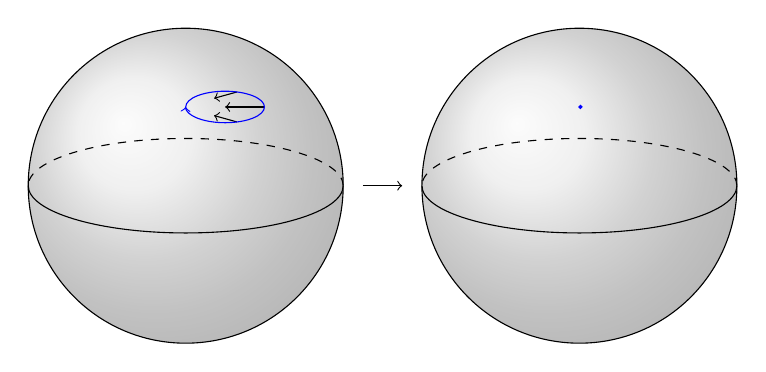
\begin{tikzpicture}
				% primera bola
				\shade[ball color = gray!40, opacity = 0.4] (0,0) circle (2cm);
				\draw (0,0) circle (2cm);
				\draw[->] (1, 1) -- (0.5,1);
				\draw[->] (0.65,1.19) -- (0.36, 1.11);
				\draw[->] (0.65,0.81) -- (0.36, 0.891);
				\draw[color = blue, ->] (0,1) arc (540:179:0.5cm and 0.2cm);
				\draw (-2,0) arc (180:360:2 and 0.6);
				\draw[dashed] (2,0) arc (0:180:2 and 0.6);
				%linea
				\draw[->] (2.25,0) -- (2.75,0);
				%segona bola
				\shade[ball color = gray!40, opacity = 0.4] (5,0) circle (2cm);
				\draw (5,0) circle (2cm);
				\draw[color = blue, fill] (5.0125,1) circle (0.02);
				\draw (3,0) arc (180:360:2 and 0.6);
				\draw[dashed] (7,0) arc (0:180:2 and 0.6);
			\end{tikzpicture}
		\end{center}
	\end{obs}

	\begin{obs}
		Existeixen corbes que no es poden contractar en un punt.
		\begin{center}
			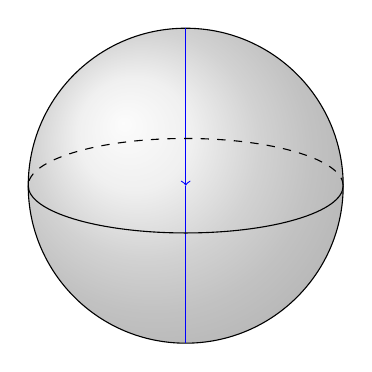
\begin{tikzpicture}
				\shade[ball color = gray!40, opacity = 0.4] (0,0) circle (2cm);
				\draw (0,0) circle (2cm);
				\draw[color = blue, ->] (0,2) -- (0,0);
				\draw[color = blue] (0,0) -- (0,-2);
				\draw (-2,0) arc (180:360:2 and 0.6);
				\draw[dashed] (2,0) arc (0:180:2 and 0.6);
			\end{tikzpicture}
		\end{center}
	\end{obs}

	\begin{obs}
		Existeixen dobles corbes que si es poden contractar en un punt.
		\begin{center}
			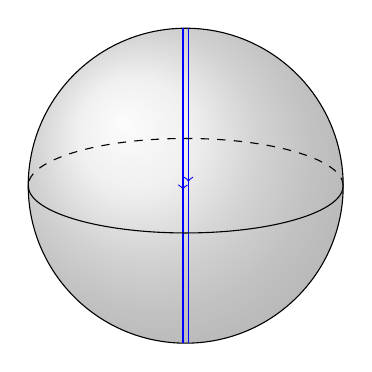
\begin{tikzpicture}
			  	\shade[ball color = gray!40, opacity = 0.4] (0,0) circle (2);
				\draw (0,0) circle (2cm);
				\draw[color = blue, ->] (0.035, 2) -- (0.035, 0.05);
				\draw[color = blue, ->] (-0.035, 2) -- (-0.035, -0.05);
				\draw[color = blue] (0.035, 0.1) -- (0.035, -2);
				\draw[color = blue] (-0.035, 0.1) -- (-0.035, -2);
				\draw (-2,0) arc (180:360:2 and 0.6);
				\draw[dashed] (2,0) arc (0:180:2 and 0.6);
			\end{tikzpicture}
		\end{center}
	\end{obs}

	Expliquem aquesta última observació:\\
	\begin{center}
		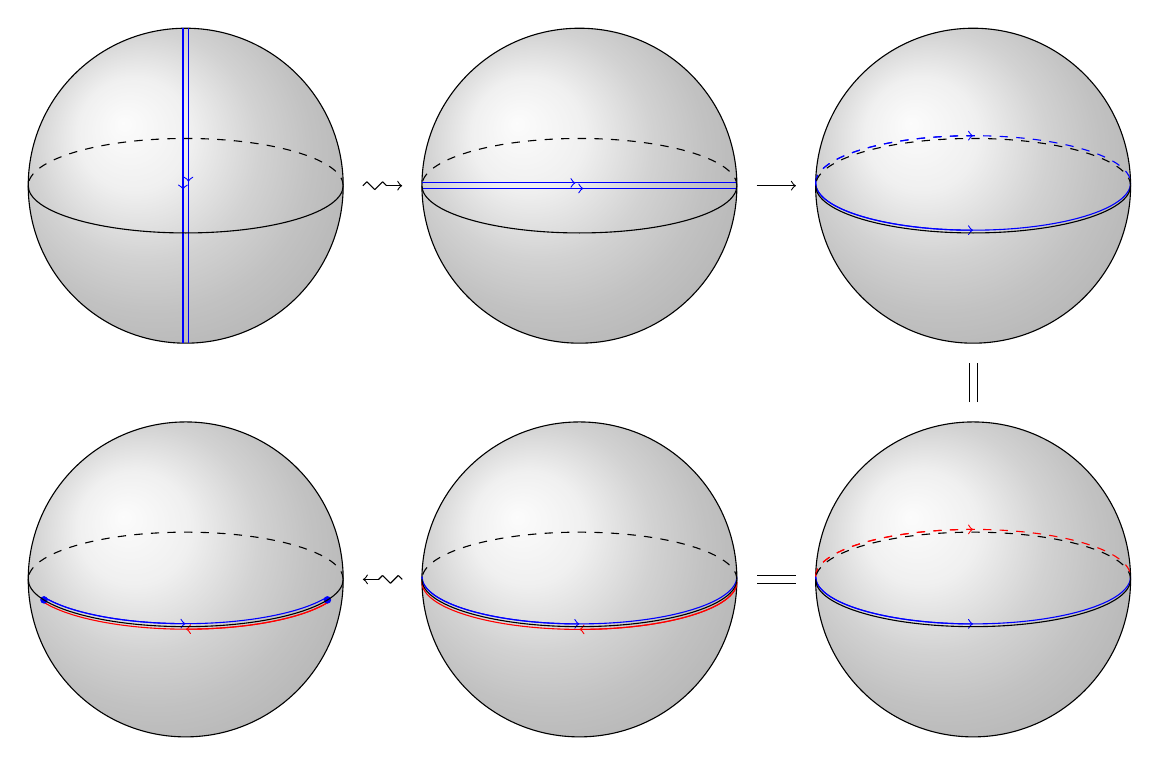
\begin{tikzpicture}
			% bola dalt esquerra
		  	\shade[ball color = gray!40, opacity = 0.4] (0,5) circle (2);
			\draw (0,5) circle (2cm);
			\draw[color = blue, ->] (0.035, 7) -- (0.035, 5.05);
			\draw[color = blue, ->] (-0.035, 7) -- (-0.035, 4.95);
			\draw[color = blue] (0.035, 5.1) -- (0.035, 3);
			\draw[color = blue] (-0.035, 5.1) -- (-0.035, 3);
			\draw (-2,5) arc (180:360:2 and 0.6);
			\draw[dashed] (2,5) arc (0:180:2 and 0.6);
		  	\shade[ball color = gray!40, opacity = 0.4] (5,5) circle (2);
			% SquigArrow (per algun motiu no funcionen llibreries que genera aquest comandament automatic)
			\draw (2.25, 5) -- (2.3, 5.05);
			\draw (2.3, 5.05) -- (2.40, 4.95);
			\draw (2.40, 4.95) -- (2.50, 5.05);
			\draw (2.50, 5.05) -- (2.55, 5);
			\draw[->] (2.55, 5) -- (2.75, 5);
			% bola dalt centre
			\draw (5,5) circle (2cm);
			\draw[color = blue] (7, 5.035) -- (4.95, 5.035);
			\draw[color = blue] (7, 4.965) -- (4.95, 4.965);
			\draw[color = blue, ->] (3, 5.035) -- (4.95, 5.035);
			\draw[color = blue, ->] (3, 4.965) -- (5.05, 4.965);
			\draw (3,5) arc (180:360:2 and 0.6);
			\draw[dashed] (7,5) arc (0:180:2 and 0.6);
			% fletxa
   			\draw[->] (7.25,5) -- (7.75,5);
			% bola dalt dreta
		  	\shade[ball color = gray!40, opacity = 0.4] (10,5) circle (2);
			\draw (10,5) circle (2cm);
			\draw[color = blue, ->] (8,5.035) arc (180:270:2 and 0.6);
			\draw[color = blue, dashed] (8, 5.035) arc (180:0:2 and 0.6);
			\draw[color = blue, dashed, ->] (8, 5.035) arc (180:90:2 and 0.6);
			\draw[color = blue] (8,5.035) arc (180:360:2 and 0.6);
			\draw (8,5) arc (180:360:2 and 0.6);
			\draw[dashed] (12,5) arc (0:180:2 and 0.6);
			% igualtat vertical
			\draw (10.05, 2.25) -- (10.05, 2.75);
			\draw (9.95, 2.25) -- (9.95, 2.75);
			% bola baix dreta
		  	\shade[ball color = gray!40, opacity = 0.4] (10,0) circle (2);
			\draw (10,0) circle (2cm);
			\draw[color = blue, ->] (8,0.035) arc (180:270:2 and 0.6);
			\draw[color = red, dashed] (8, 0.035) arc (180:0:2 and 0.6);
			\draw[color = red, dashed, ->] (8, 0.035) arc (180:90:2 and 0.6);
			\draw[color = blue] (8,0.035) arc (180:360:2 and 0.6);
			\draw (8,0) arc (180:360:2 and 0.6);
			\draw[dashed] (12,0) arc (0:180:2 and 0.6);
			% igualtat horitzontal
			\draw (7.75, 0.05) -- (7.25, 0.05);
			\draw (7.75, -0.05) -- (7.25, -0.05);
			% bola baix centre
			\shade[ball color = gray!40, opacity = 0.4] (5,0) circle (2);
			\draw (5,0) circle (2cm);
			\draw[color = blue, ->] (3,0.035) arc (180:270:2 and 0.6);
			\draw[color = red] (7, -0.035) arc (360:180:2 and 0.6);
			\draw[color = red, ->] (7, -0.035) arc (360:270:2 and 0.6);
			\draw[color = blue] (3,0.035) arc (180:360:2 and 0.6);
			\draw (3,0) arc (180:360:2 and 0.6);
			\draw[dashed] (7,0) arc (0:180:2 and 0.6);
			% SquigArrow (per algun motiu no funcionen llibreries que genera aquest comandament automatic)
			\draw (2.75, 0) -- (2.7, 0.05);
			\draw (2.7, 0.05) -- (2.6, -0.05);
			\draw (2.6, -0.05) -- (2.5, 0.05);
			\draw (2.5, 0.05) -- (2.45, 0);
			\draw[->] (2.45, 0) -- (2.25, 0);
			%bola baix esquerra
  			\shade[ball color = gray!40, opacity = 0.4] (0,0) circle (2);
			\draw (0,0) circle (2cm);
			\draw[color = blue, ->] (-1.8, -0.225) arc (206:270:2 and 0.6);
			\draw[color = red] (1.8, -0.295) arc (334:206:2 and 0.6);
			\draw[color = red, ->] (1.8, -0.295) arc (334:270:2 and 0.6);
			\draw[color = blue] (-1.8, -0.225) arc (206:334:2 and 0.6);
			\draw[color = blue, fill] (1.8, -0.26) circle (0.04cm);
			\draw[color = blue, fill] (-1.8, -0.26) circle (0.04cm);
			\draw (-2,0) arc (180:360:2 and 0.6);
			\draw[dashed] (2,0) arc (0:180:2 and 0.6);
		\end{tikzpicture}
	\end{center}

	\subsection{Els quaternions}

	En aquest nou capítol, denotarem la base ortonormal estandard $(e_1, e_2, e_3)$ a $\mathbb{R}^3$ com $(i,j,k)$.\\
	Es a dir, que $i = e_1$, $j = e_2$ i $k = e_3$.\\

	\subsubsection{Definició i primeres propietats:}

	\begin{definicio}
		Un \underline{quaternió} $q$ és la suma (formal) d'un escalar $q_0 \in \mathbb{R}$ i d'un vector $Q := (q_1, q_2, q_3) \in \mathbb{R}^3$.
		És a dir, que $q = q_0 + Q$.
		Farem servir $\mathbb{H}$ (de Hamilton) per el conjunt dels quaternions que es pot identificar a $\mathbb{R}^4$ via l'identificació:
		\begin{displaymath}
			\begin{aligned}[t]
				H &\longrightarrow \mathbb{R}^4\\
				q=q_0+q_1i+q_2j+q_3k &\longmapsto (q_0, q_1, q_2, q_3)
			\end{aligned}
		\end{displaymath}
		Denotarem també que $q = q_0 + q_1i + q_2j + q_3k$.\\
		Donats dos quaternions $p = p_0 + p_1i + p_2j + p_3k$ i $q = q_0 + q_1i + q_2j + q_3k$ i $\lambda \in \mathbb{R}$,
		definim:
		\begin{itemize}
			\item La suma de quaternions com $p + q = (p_0 + q_0) + (p_1 + q_1)i + (p_2 + q_2)j + (p_3 + q_3)k \in \mathbb{H}$
			\item El producte per un escalar com $\lambda p = \lambda p_0 + \lambda p_1i + \lambda p_2j + \lambda p_3k \in \mathbb{H}$
			\item El producte de quaternions com $\begin{aligned}[t]pq &= \underbrace{p_0q_0-\left\langle P, Q\right\rangle}_{\in \mathbb{R}} + \underbrace{p_0Q + q_0P + P \wedge Q}_{\in \mathbb{R}^3}\\pq &\in \mathbb{H}\end{aligned}$
		\end{itemize}
	\end{definicio}

	\begin{obs}
		$\forall p,q \in \mathbb{H}$,
		\begin{displaymath}
			\begin{aligned}[t]
				pq-qp   &= \left(p_0q_0-\left\langle P, Q\right\rangle\right) + \left(p_0Q + q_0P + P \wedge Q\right)\\
						& - \left(q_0p_0-\left\langle Q, P\right\rangle\right) - \left(q_0P + p_0Q + Q \wedge P\right)\\
				    	&= 2\left\langle P, Q\right\rangle
			\end{aligned}
		\end{displaymath}
	\end{obs}

	\begin{obs}
		\begin{displaymath}
			\begin{aligned}[t]
				i^2 &= ii\\
					&= (0 + 1i + 0j + 0k) (0 + 1i + 0j + 0k)\\
					&= pq \text{ amb } p_0 = q_0 = 0, p_1 = q_1 = 1, p_2 = q_2 = p_3 = q_3 = 0\\
					&= 0 - \left\langle P, Q\right\rangle + P \wedge Q\\
					&= 0 - 1 + 0\\
					&= -1
			\end{aligned}
		\end{displaymath}
		De la mateixa manera, es pot veure que $j^2 = k^2 = -1$.
	\end{obs}

	\begin{obs}
		\begin{displaymath}
			\begin{aligned}[t]
				ij &= (0 + 1i + 0j + 0k)(0 + 0i + 1j + 0k)\\
				   &= 0 - \left\langle P, Q\right\rangle + P \wedge Q\\
				   &= 0 - 0 + \begin{psmallmatrix}
							0\\0\\1
							\end{psmallmatrix}\\
				   &= k
			\end{aligned}
		\end{displaymath}
		De la mateixa manera, es pot veure que $ij = k = -ji$, $jk = i = -kj$ i $ki = j = -ik$.
	\end{obs}

	Al final, hem obtingut les regles de Hamilton, fonamentals per calcular amb quaternions:

	\begin{displaymath}
		\begin{cases}
			i^2 = j^2 = k^2 = -1\\
			ij = k = -ji\\
			jk = i = -kj\\
			ki = j = -ik
		\end{cases}
	\end{displaymath}

	En particular, veiem que $\mathbb{H}$ és un $\mathbb{R}$-espai vectorial de dimensió 4, amb base $(1, i, j, k)$ amb producte que no és conmutatiu: $ij \neq ji$!\\
	En canvi:
	\begin{proposicio}
		El producte sobre $\mathbb{H}$ és associatiu i distributiu respecte l'addicció.
	\end{proposicio}

	\begin{obs}
		$1q = q$ i $0q = 0$
	\end{obs}
	\subsubsection{Conjugació, norma i invers}
	\begin{definicio}
		Siguin $q = q_0 + \underbrace{q_1i + q_2j + q_3k}_{Q} \in \mathbb{H}$. Definim el \underline{conjugat de $q$} com
		\begin{displaymath}
			\overline{q} = q_0 - q_1i - q_2j - q_3k = q_0 - Q
		\end{displaymath}
		Direm que $q$ és:
		\begin{itemize}
			\item \underline{(quaternió) real} si $q = \overline{q} \iff Q=0 \iff q = q_0$
			\item \underline{(quaternió) imaginari pur} si $q = -\overline{q} \iff q_0 = 0 \iff q = Q$
		\end{itemize}
	\end{definicio}
	Denotem $\mathbb{R} = \left\{q \in \mathbb{H}\;\|\; \overline{q} = q \right\} \subset \mathbb{H}$ el subconjunt de reals.
	\begin{exercici}
		Demostrar que $q \in \mathbb{R} \iff pq = qp,\;\forall p \in \mathbb{H}$
	\end{exercici}
	Denotarem $\mathbb{H}^\text{pur} = \left\{q \in \mathbb{H}\;|\;\overline{q} = -q \right\} \subset \mathbb{H}$ el subconjunt de quaternions imaginaris purs.
	\begin{proposicio}
		$\forall p,q \in \mathbb{H},\; \overline{p+q} = \overline{p} + \overline{q}\text{ i }\overline{pq} = \overline{q}\overline{p}$
	\end{proposicio}
	\begin{demostracio}
        El primer punt és evident. Pel segon, ja n'hi ha prou donada la distribuitivitat de verificar-ho per $i, j, k$ i per exemple:
        \begin{displaymath}
        	\begin{cases}
	       		\overline{ij} = \overline{k} = -k\\
	         	\overline{j}\overline{i} = -j(-i) = ji = -k\\
			\end{cases}
		\end{displaymath}
	\end{demostracio}
	\begin{definicio}
		Sigui $q \in \mathbb{H}$. Definim la seva norma $N(q) \in \mathbb{R}_+$ per la fòrmula:
		\begin{displaymath}
			N(q) = \sqrt{q\overline{q}} \in \mathbb{R}
		\end{displaymath}
	\end{definicio}
	\begin{obs}
	    $\overline{q\overline{q}} = \overline{q\overline{q}} \Rightarrow q\overline{q} \in \mathbb{R}$ i a més
		\begin{displaymath}
			\begin{aligned}[t]
				q\overline{q} &= (q_0 + q_1i + q_2j + q_3k)(q_0 - q_1i - q_2j - q_3k)\\
							  &= q_0^2 - \left\langle Q, -Q\right\rangle + \underbrace{q_0\left(-Q\right) + q_0\left(Q\right)}_{=0} + \underbrace{Q \wedge (-Q)}_{=0}\\
							  &= q_0^2 + \left\langle Q, Q\right\rangle\\
			\end{aligned}
		\end{displaymath}
		es a dir $q\overline{q} = q_0^2+q_1^2+q_2^2+q_3^2 \in \mathbb{R}_+$
	\end{obs}
	En particular, $N(q) \geq 0$ i $ N(q) = 0 \iff q = 0$.
	\begin{obs}
		$N(q)$ coincideix amb la norma euclidiana a $\mathbb{R}^4$ per la identificació
		\begin{displaymath}
			\begin{aligned}[t]
				\mathbb{H} &\simeq \mathbb{R}^4\\
				1 &\leftrightarrow e_1\\
				i &\leftrightarrow e_2\\
				j &\leftrightarrow e_3\\
				k &\leftrightarrow e_4
			\end{aligned}
		\end{displaymath}
	\end{obs}
	\begin{proposicio}
		La norma $N : \mathbb{H} \to \mathbb{R}_+$ es multiplicativa, és a dir, $N(pq) = N(p)N(q)\;\forall p,q \in \mathbb{H}$.
	\end{proposicio}
	\begin{demostracio}
		\begin{displaymath}
			N^2(pq) = pq\overline{pq} = \overline{q}\underbrace{\overline{p}p}_{N^2(p)}q = \underbrace{q}N^2(p)q = N^2(p)N^2(q)
		\end{displaymath}
	\end{demostracio}
	\begin{obs}
		Denotem
		\begin{displaymath}
			\begin{aligned}[t]
				\mathbb{C} &= \left\{q \in \mathbb{H} \text{ tal que } q_2 = q_3 = 0\right\}\\
						   &= \left\{q_0 + q_1i | q_0, q_1 \in \mathbb{R}\right\}
			\end{aligned}
		\end{displaymath}
		Obeeix que $\mathbb{C}$ és estable per la multiplicació.
		Tenim llavors que $\mathbb{R} \subset \mathbb{C} \subset (\mathbb{H}, +, \times)$
	\end{obs}
	\begin{definicio}
		Sigui $q \in \mathbb{H}$ i $q \neq 0$, aleshores, la inversa de $q$, $q^{-1} = \frac{\overline{q}}{N(q)^2}$ que compleix $q^{-1}q = 1$ i $qq^{-1} = 1$.
	\end{definicio}
	\begin{teorema}
	    $\mathbb{H}$ és un cos (com $\mathbb{R}\text{ i }\mathbb{C}$).
	\end{teorema}
	\begin{demostracio}
	\begin{itemize}
			\item La suma i la multiplicació són associatives.
			\item La suma és commutativa.
			\item Existeix element neutre per la suma i per la multiplicació ($0$ i $1$, respectivament).
			\item Distribució de multiplicació relativa a suma.
			\item Tot element admet un invers per la suma ($q+(-q) = 0$).
			\item Tot element no nul admet un invers per la multiplicació ($qq^{-1} = 1$).
		\end{itemize}
	\end{demostracio}
	\begin{notacio}
		Si $q \in \mathbb{H},\;Re\;q := \frac{1}{2}\left(q + \overline{q}\right) \in \mathbb{R}$ i $Im\;q := \frac{1}{2}\left(q - \overline{q}\right) \in \mathbb{H}^{pur}$.\\
	\end{notacio}
	\subsubsection{Quaternions unitaris}
	\begin{definicio}
		Un quaternió $u \in \mathbb{H}$ és unitari si satisfà $N(u) = 1$. Denotarem $\mathbb{H}^* = \left\{q \in \mathbb{H} | N(q) = 1\right\}$ el conjunt dels quaternions unitaris.
		Denotarem $\mathbb{U} = \left\{u \in \mathbb{H}\;\|\;N(u) = 1\right\}$ el subconjunt dels quaternions unitaris.
	\end{definicio}
	Aquest subconjunt té les següents propietats:
	\begin{proposicio} $\;$
		\begin{enumerate}
			\item $\forall u, v \in \mathbb{U},\;u^{-1} = \overline{u}$ i $uv \in \mathbb{U}$ i en particular,
			$(\mathbb{U}, \times)$ satisfà les propietats d'un grup.
			\item $\mathbb{U} \cap \mathbb{R} = \left\{\pm 1\right\}$
		\end{enumerate}
	\end{proposicio}
	\begin{demostracio}
		\begin{enumerate}
			\item $\forall u \in \mathbb{U}\; u^-1 = \overline{u}$ ja que $N(u) = 1$, aleshores $N(\overline{u}) = N(\overline{u})N(u) = N(u\overline{u}) = 1 \Rightarrow u^{-1}\in \mathbb{U}$
			\item Si $u \in \mathbb{R}\;u = u_0$ amb $u_0 \in \mathbb{R}$ i $N^2(u) = u_0^2 = 1 \Rightarrow u = u_0 = \pm 1$
		\end{enumerate}
	\end{demostracio}
	\begin{obs}
		Podem escriure $\mathbb{U} = \left\{q_0+q_1i+q_2j+q_3k | (q_0, q_1, q_3, q_4) \in \mathbb{R}^4\text{ i } q_0^2 + q_1^2 + q_3^2 + q_4^2 \right\}$,
		i observem que
		\begin{displaymath}
			\begin{aligned}[t]
				\mathbb{H} &\tilde{\longleftrightarrow} R^4\\
				\breve{\mathbb{U}} &\tilde{\longleftrightarrow} \breve{S^3}
			\end{aligned}
		\end{displaymath}
		$\mathbb{U}$ s'identifica amb l'esfera $\mathbb{S}^3 \subset \mathbb{R}^4$
	\end{obs}
	Recordem que $\begin{aligned}[t]
					\mathbb{H}^{pur} &= \left\{q \in \mathbb{H} | \overline{q} = -q\right\}\\
									 &= \left\{q \in \mathbb{H} | Re\;q = 0\right\}\\
									 &= \left\{Q | Q \in \mathbb{R}^3\right\}
				  \end{aligned}$
	i per aixó podem identificar $\mathbb{H}^{pur}$ amb $\mathbb{R}^3$ via l'aplicació
	\begin{displaymath}
		\begin{aligned}[t]
			\mathbb{H}^{pur} &\to \mathbb{R}^3\\
			q = Q = q_1i + q_2j + q_3k &\mapsto Q = (q_1, q_2, q_3)
		\end{aligned}
	\end{displaymath}
	\begin{proposicio}
		Si $q = Q \in \mathbb{H}^{pur},\; q^2 = -N^2(q) = -\left\lVert Q \right\rVert^2$
	\end{proposicio}
	\begin{demostracio}
		Si $p, q \in \mathbb{H}^{pur},\; pq = -\left\langle P, Q \right\rangle + P\wedge Q$ com $p_0 = q_0 = 1$ i en particular
		\begin{displaymath}
			q^2 = -\left\langle Q, Q \right\rangle = -\left\lVert Q \right\rVert^2 = - N^2(q)
		\end{displaymath}
	\end{demostracio}
	\begin{obs}
		Si $p,q \in \mathbb{H}^{pur},\; pq-qp = 2 P\wedge Q$
	\end{obs}
	\begin{teorema}
		Siguin $p, q, r \in \mathbb{H}^{pur}$ i denotem els vectors corresponents per $P, Q, R \in \mathbb{R}^3$. Aleshores
		\begin{displaymath}
			(P, Q, R) \text{ BON } \oplus \text{ a } \mathbb{R}^3 \Leftrightarrow \begin{cases}
				p^2 = q^2 = r^2 = -1\\
				pq = r = -qp\\
				qr = p = -rq\\
				rp = q = -pr
				\end{cases}
		\end{displaymath}
	\end{teorema}
	\begin{obs}
		$(i, j, k)$ compleixen aquestes formules! No es sorpresa ja que $(i, j, k)$ és un BON $\oplus$ a $\mathbb{R}^3$.
	\end{obs}
	\begin{demostracio}
		$\left(\Leftarrow\right)$ Recordem que si $q \in \mathbb{H}^{pur},\; q^2 = -N^2(q) = -\left\lVert Q \right\rVert^2$ i per tant $P,Q,R$ són de norma euclidiana $=1$
		\begin{lema}
			Si $p,q \in \mathbb{H}^{pur},\text{i}\; P,Q \in \mathbb{R}^3$ són els vectors associats aleshores
			\begin{displaymath}
				\begin{cases}
					Re\left(pq\right) &= -\left\langle P, Q \right\rangle\\
					Im\left(pq\right) &= P\wedge Q
				\end{cases}
			\end{displaymath}
		\end{lema}
		\begin{demostracio}
			$pq = p_0q_0 - \left\langle P, Q \right\rangle +p_0Q+q_0P + P\wedge Q = -\left\langle P, Q \right\rangle + P\wedge Q$ ja que $p_0 = q_0 = 0$
		\end{demostracio}
		Ara bé, $P\wedge Q = pq = r = R$ i $\left\langle P, Q \right\rangle = -Re(pq) = -Re(r) = 0$ doncs $\left(P,Q,R\right)$ BON directe.
		$\left(\Rightarrow\right)$ Si $\left(P,Q,R\right)$ és BON $\oplus,\; \left\lVert P \right\rVert = 1 = -p^2$ i idem per $Q$ i $R$. Aleshores $pq = - \underbrace{\left\langle P, Q \right\rangle}_{=0} + P\wedge Q = R = r$ i idem per $qr$ i $rp$.
	\end{demostracio}
	\subsubsection{Quaternions i Rotacions}
	Sigui $u \in \mathbb{U}$, considerem l'aplicació $\begin{aligned}[t]\Phi_u: \mathbb{H} &\to \mathbb{H}\\q &\mapsto uq\overline{u}\end{aligned}$
	\begin{proposicio}
		$\forall p, q \in \mathbb{H},\;\forall \lambda \in \mathbb{R}$
		\begin{enumerate}
			\item $\Phi_u$ és lineal: $\Phi_u(p + \lambda q) = \Phi_u(p) + \lambda\Phi_u(q)$
			\item $\Phi_u$ és multiplicativa: $\Phi_u(pq) = \Phi_u(p)\Phi_u(q)$
			\item $\overline{\Phi_u(p)} = \Phi_u(\overline{p})$
			\item $Re(\Phi_u(p)) = Re(p)$, en general $Im(\Phi_u(p)) \neq Im(p)$
			\item $\Phi_u$ preserva la norma: $N(\Phi_u(p)) = N(p)$
		\end{enumerate}
	\end{proposicio}
	\begin{demostracio}
		1 i 2 son clares.
		\begin{enumerate}\addtocounter{enumi}{2}
			\item $\overline{uq\overline{u}} = \overline{\overline{u}}\overline{q}\overline{u} = u\overline{q}\overline{u}$
			\item $Re(q) := \frac{1}{2}(q + \overline{q}) \rightsquigarrow Re(\Phi_u(p)) \begin{aligned}[t]
				&= \frac{1}{2}(\Phi_u(p) + \overline{\Phi_u(p)}) =  \frac{1}{2}(\Phi_u(p) + \Phi_u{\overline{p}})\\
				&= \Phi_u(Re p) = Re(p \Phi_u(1))\\
				&= Re(p)
			\end{aligned}$
			\item $N(\Phi_u(p)) = \sqrt{up\overline{u}u\overline{p}\overline{u}} = \sqrt{up\overline{p}\overline{u}} = N(p)$
		\end{enumerate}
	\end{demostracio}
	A més:
	\begin{proposicio} $\forall u,v \in \mathbb{U}$
		\begin{itemize}
			\item $\Phi_u = Id_\mathbb{H} \iff u = \pm 1$
			\item $\forall u, v \in \mathbb{U}, \Phi_{uv} = \Phi_u \circ \Phi_v$ i $\Phi_u$ és invertible, amb $\Phi_u^{-1} = \Phi_{\overline{u}}$
			\item $\Phi_u = \Phi_v \iff u = \pm v$
		\end{itemize}
	\end{proposicio}
	\begin{demostracio}
		\begin{enumerate}
			\item Si $u = \pm 1$ aleshores $\Phi_u = Id_\mathbb{H}$ Reciprocament, si $\Phi_u = Id_\mathbb{H}$ aleshores $\forall q \in \mathbb{H},\; uq\overline{u} = q \iff u\overline{q} = qu$
			\begin{lema}
				Si $p \in \mathbb{H}$, tal que $\forall q \in \mathbb{H}, pq = qp$ aleshores $p \in \mathbb{R}$.
			\end{lema}
			\begin{demostracio}
				Escribim $p = p_0 + p_1i + p_2j + p_3k$. En particular,
				\begin{displaymath}
					\begin{aligned}[t]
						pi = ip &\iff p_0i - p_1 - p_2k - p_3j = p_0i - p_1 + p_2k + p_3j\\
						&\iff 2p_2k + 2p_3j = 0\\
						&\iff p_2 = p_3 = 0 \iff p = p_0 + p_1i
					\end{aligned}
				\end{displaymath}
				i la relació $pj = jp \iff p_1 = 0$. Al final $p = p_0 \in \mathbb{R}$.
			\end{demostracio}
			Doncs $u \in \mathbb{R}\cap\mathbb{U} \{\pm 1\}$.
			\item $\Phi_u(\Phi_v(p)) = uvp\overline{v}\overline{u} = uvp\overline{uv} = \Phi_{uv}(p)$
			Ara bè, $\forall u \in \mathbb{U},\;\Phi_u\circ\Phi_{\overline{u}} = \Phi_{u\overline{u}} = \Phi_1 = Id_\mathbb{H} \Rightarrow \Phi_{u}^{-1} = \Phi_{\overline{u}}$
			\item $\Phi_u = \Phi_v \Rightarrow \Phi_u \circ \Phi_{v^{-1}} = Id_\mathbb{H}$
		\end{enumerate}
	\end{demostracio}
	Ara denotarem $\begin{aligned}[t]\Psi_u: \mathbb{H}^{pur} &\to \mathbb{H}^{pur}\\q &\mapsto uq\overline{u}\end{aligned}$ la restricció de $\Phi_u$ als quaternions imaginaris purs.\\
	Si identifiquem $\begin{aligned}[t]\mathbb{H}^{pur} &\simeq \mathbb{R}^3\\p_1i+p_2j+p_3k &\tilde{\mapsto} (p_1, p_2, p_3)\end{aligned}$, obtenim una aplicació induïda $R_u: \mathbb{R}^3 \to \mathbb{R}^3$ definit per $R_u(p_1, p_2, p_3) = \Psi_u(p_1i+p_2j+p_3k)$\\
	Les dues proposicions anteriors impliquen el següent:
	\begin{itemize}
		\item $R_u$ és lineal $\forall p,q \in \mathbb{R}^3,\;\forall\lambda\in\mathbb{R}$
		\item $R_u$ és invertible
		\item De fet, $R_u$ serà una rotació.
	\end{itemize}
	\begin{teorema}
		$u, v \in \mathbb{U}$, aleshores
		\begin{enumerate}
			\item $R_u \in SO(3)$ (és a dir, $R_u$ és una rotació)
			\item $R_u \circ R_v = R_{uv}$ i $R_u^{-1} = R_{\overline{u}}$
			\item $R_u = R_v \iff u = \pm v$
		\end{enumerate}
	\end{teorema}
	\begin{demostracio}
		\begin{enumerate}
			\item Observem que $\Psi_u(i^2) = \Psi_u(i)^2 \iff -1 = \Psi_u(i)^2$ i de la mateixa manera $\Psi_u(j)^2=\Psi_u(k)^2 = -1$.
			Després $\Psi_u(ij)=\Psi_u(k)=\Psi_u(-ji) \iff \Psi_u(i)\Psi_u(j) = \Psi_u(k) = -\Psi_u(j)\Psi_u(i)$ i de la mateixa manera obtenim
			\begin{displaymath}
				\begin{cases}
					\Psi_u(j)\Psi_u(k) = \Psi_u(i) = -\Psi_u(k)\Psi_u(j)\\
					\Psi_u(k)\Psi_u(i) = \Psi_u(j) = -\Psi_u(i)\Psi_u(k)
				\end{cases}
			\end{displaymath}
			I doncs deduim que $\left(\Psi_u(i), \Psi_u(j), \Psi_u(k)\right)$ és un BON $\oplus$ de $\mathbb{R}^3 \Rightarrow (R_u(1,0,0), R_u(0,1,0), R_u(0,0,1))$ és un BON $\oplus \Rightarrow mat_{(e_1, e_2, e_3)}(R_u) \in SO(3)$.
		\end{enumerate}
		2 i 3 es dedueixen de la proposició anterior.
	\end{demostracio}
	\begin{notacio}
		Des d'ara no distingirem entre $R_u$ i $\Psi_u$.
	\end{notacio}
	\begin{obs}
		En particular, obtenim un morfisme de grups:
		\begin{displaymath}
			\begin{aligned}[t]
				R: (\mathbb{U}, \times) &\to (SO(3), \times)\\
				u &\mapsto R_u (= \Psi_u \text{ via la identificació} \mathbb{R}^3 \simeq \mathbb{H}^{pur})
			\end{aligned}
		\end{displaymath}
		Amb $R_u(Q) = R_u(q) = uq\overline{u}$\\
		tal que $R_{uv} = R_u \circ R_v$ i $R_u = R_v \iff u = \pm v$.\\
		Aixi podem identificar $SO(3) \simeq \mathbb{U}\bigslant\{\pm Id\} \simeq \mathbb{S}^3\bigslant\{\pm 1\}$.
	\end{obs}
	Ara veiem que $R$ és exhaustiva i permet descriure qualsevol rotació.
	\begin{teorema}
		Sigui $Q = (q_1, q_2, q_3) \in \mathbb{R}^3$ amb $\left\lVert Q \right\rVert = 1$, $\theta \in \mathbb{R}$.\\
		Definim $u(Q, \theta) = \cos{\frac{\theta}{2}} + \sin{\frac{\theta}{2}}Q$. Aleshores $u(Q, \theta) \in \mathbb{U}$ i $R_{u(Q, \theta)}$ és la rotació a $\mathbb{R}^3$ d'un eix $Q$ i un angle $\theta$. En particular, l'aplicació $R$ és exhaustiva.
	\end{teorema}
	\begin{demostracio}
		\begin{displaymath}
			\begin{aligned}[t]
				N(u(Q, \theta)) &= u(Q, \theta) \overline{u(Q, \theta)}\\
								&= \cos^2{\frac{\theta}{2}} - \sin^2{\frac{\theta}{2}} Q^2\\
								&= \cos^2{\frac{\theta}{2}} + \sin^2{\frac{\theta}{2}}\\
								&= 1
			\end{aligned}
		\end{displaymath}
		Primer, comprovem que $q = Q \in \mathbb{H}^{pur}$ és l'eix de la rotació $R_{u(Q, \theta)}$:\\
		\begin{displaymath}
			\begin{aligned}[t]
				R_{u(Q, \theta)}(q) &= (\cos{\frac{\theta}{2}} + \sin{\frac{\theta}{2}}Q)Q(\cos{\frac{\theta}{2}} - \sin{\frac{\theta}{2}}Q)\\
									&= \underbrace{(\cos{\frac{\theta}{2}} + \sin{\frac{\theta}{2}}Q)(\cos{\frac{\theta}{2}} - \sin{\frac{\theta}{2}}Q)}_{ = u(Q, \theta)\overline{u(Q, \theta)}}
									&= Q \iff R_{u(Q, \theta)}(Q) = Q
			\end{aligned}
		\end{displaymath}
		Ara comprovem que l'angle de la rotació $R_{u(Q,\theta)}$ és $\theta$:\\
		Per això triem $P_1, P_2 \in \mathbb{R}^3 \rightsquigarrow p_1, p_2 \in \mathbb{H}^{pur}$ tals que $(P_1, P_2, Q)$ sigui BON $\oplus$.\\
		Com $P_1, P_2, Q$ és BON $\oplus$ calculem
		\begin{displaymath}
			\begin{aligned}[t]
				R_{u(Q, \theta)}(P_1)
									&= (\cos{\frac{\theta}{2}} + \sin{\frac{\theta}{2}}Q)P_1(\cos{\frac{\theta}{2}} - \sin{\frac{\theta}{2}}Q)\\
									&= (\cos{\frac{\theta}{2}} + \sin{\frac{\theta}{2}}Q)(\cos{\frac{\theta}{2}}P_1 - \sin{\frac{\theta}{2}}\underbrace{P_1Q}_{=-QP_1})\\
									&= (\cos{\frac{\theta}{2}} + \sin{\frac{\theta}{2}}Q)(\cos{\frac{\theta}{2}}P_1 + \sin{\frac{\theta}{2}}Q)P_1\\
									&= (\cos^2{\frac{\theta}{2}} + \sin{\frac{\theta}{2}}\cos{\frac{\theta}{2}}Q + \sin{\frac{\theta}{2}}\cos{\frac{\theta}{2}}Q + \sin^2{\frac{\theta}{2}}Q)P_1\\
									&= (\cos^2{\frac{\theta}{2}} - \sin^2{\frac{\theta}{2}})P_1 + 2\sin{\frac{\theta}{2}}\cos{\frac{\theta}{2}}\underbrace{QP_1}_{=P_2}\\
									&= \cos{\theta}P_1 + \sin{\theta}P_2
			\end{aligned}
		\end{displaymath}
		Per tant, deduim que l'angle de $R_{u(Q, \theta)}$ és $\theta$.
	\end{demostracio}
	\begin{obs}
		Podem comprovar que $R_{u(Q, \theta)(P_2) = -\sin{\theta}}P_1 + \cos{\theta}P_2$.
		Deduïm que
		\begin{displaymath}
			Mat_(Q, P_1, P_2)(R_{u(Q, \theta)}) = \begin{pmatrix}
				1 & 0 & 0\\
				0 & \cos{\theta} & -\sin{\theta}\\
				0 &\sin{\theta} & \cos{\theta}\\
			\end{pmatrix}
		\end{displaymath}
	\end{obs}
	\subsection{Interpolació de rotacions}
	Pregunta: Si tenim dos punts de vista sobre una situació: aquí tenim dos matrius $A_0$ i $A_1 \in SO(3)$. Com podem pasar d'un punt de vista (camera 0) a l'altre punt de vista (camera 1)?\\
	De forma equivalent, busquem una familia de matrius
	\begin{displaymath}
		\{A_t\}_{t\in[0,1]}\;tq\;\begin{cases}
			A_0 = \overline{A_0}\\
			A_1 = \overline{A_1}\\
			(t \mapsto A_t \text{ es contiuna})
		\end{cases}
		\text{ i } A_t \in SO(3)\;\forall t \in [0,1]
	\end{displaymath}
	Trobar la familia $\{A_t\}_{t\in[0,1]}$ se'n diu fer la interpolació entre $\overline{A_0}$ i $\overline{A_1}$.\\
	Sabem inicialment que aquesta interpolació sempre existeix, i a més no és única.\\
	Aquest problema es díficil, com busquem els $9$ coeficients de $A_t$ que han de satisfer les equacions següents:
	\begin{displaymath}
		\begin{cases}
			A_t^tA_t = I &\text{(6 quadratiques per simetria)}\\
			\det{A_t} = 1 &\text{(1 cúbica)}
		\end{cases}
	\end{displaymath}
	Pero ho podem fer "fàcilment" fent servir els quaterinons.\\
	Com ho fem?\\
	Primer representem $\overline{A_0}$ i $\overline{A_1} \in SO(3)$ amb quaternions unitaris:
	\begin{displaymath}
		\exists u, v \in \mathbb{U}\;tq\;\overline{A_0} = R_u \text{ i } \overline{A_1} = R_v
	\end{displaymath}
	Sigui $w \in Vect(u, v) \cap \mathbb{U}$ tal que
	\begin{displaymath}
		\begin{cases}
			\left\langle u, w \right\rangle = 0\\
			\left\langle v, w \right\rangle = 0
		\end{cases}
	\end{displaymath}
	$\exists \theta \in [0, \pi)$ tq $v = \cos{\theta}u + \sin{\theta}w$\\
	Aleshores obtenim que
	\begin{displaymath}
		\begin{aligned}[t]
			&q := v\overline{u} = (\cos{\theta} + \sin{\theta}w)\overline{u} \in \mathbb{U}\\
			\iff & q = \cos{\theta} + \sin{\theta}w\overline{u}\\
			\iff & w = \frac{v - \cos{\theta}u}{\sin{\theta}}
		\end{aligned}
	\end{displaymath}
	Finalment, posem $\forall t \in [0,1],\;U_t := \cos{t\theta}u + \sin{t\theta}w \in \mathbb{U}$ i com $u_0 = u$ i $u_1 = v$, deduïm que $A_t := R_{U_t} (\forall t \in [0,1])$ ens defineix una interpolació entre $\overline{A_0}$ i $\overline{A_1}$.\\
	Com trobar $w$ i $\theta$ en la pràctica?\\
	Busquem $\theta \in [0, \pi)$ i $q \in \mathbb{U}$ tq $vu^{-1} = \cos{\theta} + \sin{\theta}q$.\\
	Aleshores tenim el $\theta$ buscat i obtenim
	\begin{displaymath}
		w = qu\;(= \frac{v - \cos{\theta}u}{\sin{\theta}})
	\end{displaymath}
	Ara expliquem que son els angles d'Euler.\\
	\begin{teorema}
		Posem $\forall \alpha, \beta, \gamma \in \mathbb{R}$,
		\begin{displaymath}
			\begin{cases}
				R_{i}(\alpha) :=\begin{pmatrix}
					1 & 0 & 0\\
					0 & \cos{\alpha} & -\sin{\alpha}\\
					0 & \sin{\alpha} & \cos{\alpha}
				\end{pmatrix}\\
				R_{j}(\beta) :=\begin{pmatrix}
					\cos{\beta} & 0 & \sin{\beta}\\
					0 & 1 & 0\\
					-\sin{\beta} & 0 & \cos{\beta}
				\end{pmatrix}\\
				R_{k}(\gamma) :=\begin{pmatrix}
					\cos{\gamma} & -\sin{\gamma} & 0\\
					\sin{\gamma} & \cos{\gamma} & 0\\
					0 & 0 & 1
				\end{pmatrix}
			\end{cases}
		\end{displaymath}
		Aquestes matrius generen totes les rotacions a l'espai:\\
		$\forall A \in SO(3),\; \exists \alpha, \beta, \gamma \in \mathbb{R}$
		anomenats angles d'Euler, tal que\\
		$A = R_{i}(\alpha)R_{j}(\beta)R_{k}(\gamma)$
	\end{teorema}
\end{document}
